%\vspace{-0.1in}
\section{Introduction}
\label{sec:intro}

Public cloud providers like Microsoft and Google are deploying Remote Direct
Memory Access (RDMA) over Ethernet (RoCE) in their data centers to enable low
latency, high throughput data transfers with minimal CPU
overhead~\cite{dcqcn,timely}. Systems like Pilaf~\cite{pilaf}, Farm~\cite{farm},
TesnorFlow~\cite{tensorflow}, and CNTK~\cite{cntk} rely on RDMA/RoCE for
enhanced performance. 

RoCE uses Priority Flow Control (PFC) to prevent packet drops due to buffer
overflow at the switches. PFC allows a switch to temporarily pause its upstream
neighbor. While PFC is effective, it can lead to
deadlocks~\cite{rdmaatscale,tcpbolt,hu2016deadlocks}. Deadlocks are caused by
circular buffer dependency (CBD)~\cite{hu2016deadlocks}, {\em i.e.,} the occupied 
buffers are waiting for each other in a loop.

While CBD can be caused by a routing loop, routing loop is not required -- flows
that travel on loop-free paths can create buffer dependencies that lead to CBD.
A simple but contrived example is shown in Figure~\ref{fig:basic_deadlock}. We
will discuss more realistic scenarios (e.g. Figure~\ref{fig:clos_1_bounce})
later.  See~\cite{hu2016deadlocks} for several other examples. 

The deadlock problem is not merely theoretical -- our conversations with
engineers at large cloud providers confirm that they have seen the problem in
practice and at least one provider has reported it publicly~\cite{rdmaatscale}.
Deadlock is a serious problem because a deadlock is not transient -- once a
deadlock forms, it does not go away even after the conditions (e.g. a temporary
routing loop due to link failure) that caused its formation have
abated~\cite{rdmaatscale}. Worse, a small initial deadlock may cause the PFC
frames to propagate and create a global deadlock, and shutdown the whole
network.

Current solutions to the deadlock problem fall in two categories. The first
category consists of solutions that {\em detect} the formation of the deadlock
and then use various techniques to {\em break} it~\cite{shpiner2016unlocking}.
These solutions do not address the root cause of the problem, and hence cannot
guarantee that the deadlock would not immediately reappear.

The second category of solutions are designed to {\em prevent} deadlocks.  For
deadlock formation, CBD is {\em necessary}, but not {\em
sufficient}~\cite{hu2016deadlocks}. Unfortunately, {\em sufficient} conditions
for deadlock formation are not well understood~\cite{hu2016deadlocks}. Thus,
currently, preventing CBD is the only practical way to prevent deadlocks.

In \S\ref{sec:challenges}, using data from a large cloud provider's data
centers, we show that any practical deadlock prevention scheme must meet three
key challenges. These include: $(i)$ it should require no changes to existing
routing protocols or switch hardware, $(ii)$ it must deal with link failures and
associated  route changes, and $(iii)$ it must work with limited buffer
available in commodity switches.

Prior proposals for deadlock prevention fail to meet one or more of these
challenges.  Some schemes~\cite{infiniband,blazewicz1994optimal} require
centralized routing.  These are difficult to deploy in existing data centers.
Others are distributed, but brand-new routing
protocols~\cite{dally,duato93,dally93,sancho2004,flich2012survey,lash,wu2003fault,glass,duato2001,domke2011,puente1999,dfedst16,tcpbolt,dfedst16}
that are not supported by commodity switches.  Many of these schemes also
require carefully controlling the paths -- something that is simply not possible
with decentralized routing in presence of link failures~\cite{netpilot}.
Finally, some schemes~\cite{firstpaper,survey,datanetworks,karol2003prevention},
require creation of numerous priorities and buffer management according to those
priorities.  However, modern data center networks, built using commodity
switches, can realistically support only two or three lossless
priorities~\cite{rdmaatscale}.

In this paper, we present \sysname{}, which meets all three challenges described
above. \sysname{} is based on a simple observation: in a data center, we can ask
the operator to supply a list of paths that must be lossless.  We call these
expected lossless paths (ELPs). Enumerating ELPs is straightforward for
``structured'' topologies like Clos~\cite{clos}, FatTree~\cite{fattree} or
Bcube~\cite{bcube}, and not onerous even for randomized topologies like
Jellyfish~\cite{jellyfish}.

Using ELPs, we create a system of match-action rules to ``tag'' packets. The
switches use these tags to enqueue packets in different lossless queues. The
tags carried in packets are manipulated in a way such that CBD never forms due
to packets traveling on paths in ELP.  If packets ever deviate from paths in ELP
(e.g. due to link failures or routing errors) they are automatically placed in a
lossy queue to ensure that they do not trigger PFC. \sysname{} guarantees that
there will be no deadlock - even under unforeseen link failures or routing
errors. Even routing loops won't lead to deadlock!

\sysname{} works for any routing protocol because there are no restrictions on
what paths can be included in the ELP, tagging rules are static, and are
specified only in terms of local information (tag, ingress port and egress port)
available at each switch.

The number of lossless queues and the number of tag match-action rules required
by \sysname{} are small.  Even for a Jellyfish topology with 2000 switches,
\sysname{} requires just three lossless queues per switch.  In fact, we prove
that for Clos topology,  \sysname{} is optimal in terms of number of lossless
queues required.  We also show how to minimize the number of match-action rules
required to implement \sysname{}.

We have implemented and tested \sysname{} on commodity Arista 7050 Switches with
Broadcom chipsets. The implementation requires carefully addressing the problem
of priority transition (\S\ref{sec:implementation}). Our tests show that
\sysname{} has no impact on throughput and latency of RDMA traffic.

\begin{figure}[t]
		\centering
		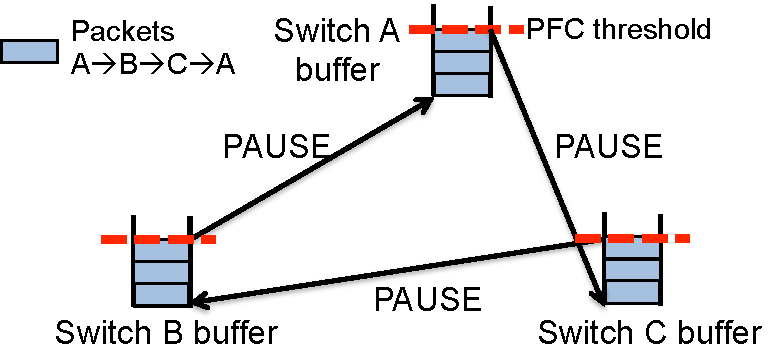
\includegraphics[width=0.45\textwidth] {figs/deadlock}
		\vspace{-1em}
		\caption{A simple (but contrived) example to illustrate CBD formation
		without routing loop.}
		\vspace{-1em}
		\label{fig:basic_deadlock}
\end{figure}
